\documentclass{article}

\usepackage{amsmath}
\usepackage{float}
\usepackage{graphicx}

\usepackage[colorlinks=true, allcolors=blue]{hyperref}

\title{Lista 1}
\author{Luís Felipe Ramos Ferreira}
\date{\href{mailto:lframos.lf@gmail.com}{\texttt{lframos.lf@gmail.com}}
}

\begin{document}

\maketitle

\begin{enumerate}

	\item Capítulo lido
	      %imagem de trabalho feito
	\item
	      \begin{itemize}
		      \item (1.5.3)
		            \begin{enumerate}
			            \item
			                  \begin{figure}[H]
				                  \centering
				                  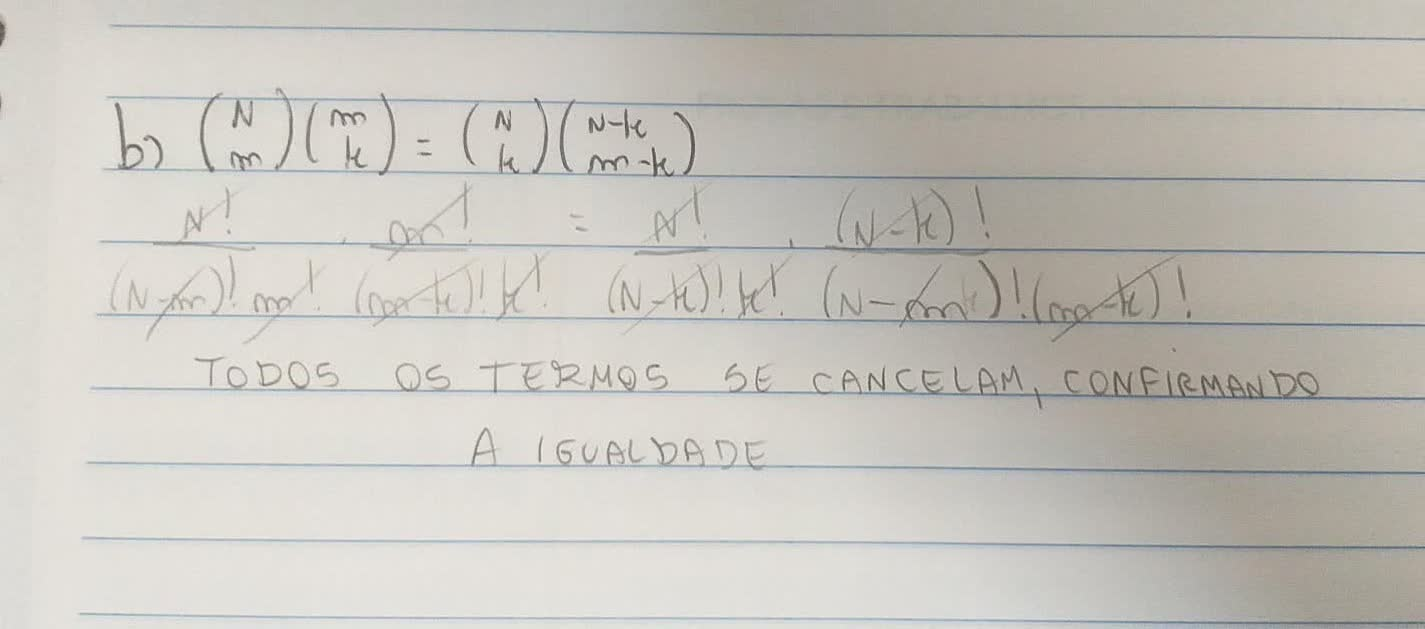
\includegraphics[width=0.8\textwidth]{images/153b.jpg}
				                  \caption{Questão 1.5.3 - a)}
			                  \end{figure}
			            \item
			                  \begin{figure}[H]
				                  \centering
				                  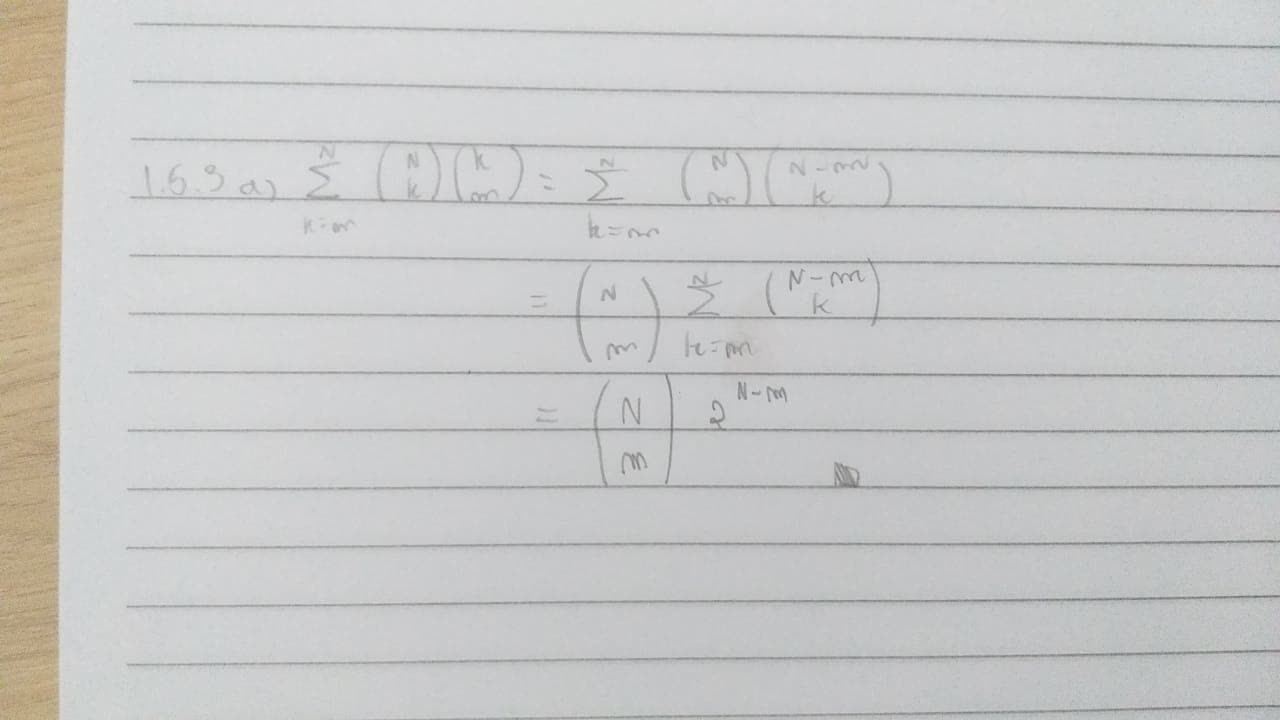
\includegraphics[width=0.8\textwidth]{images/153a.jpg}
				                  \caption{Questão 1.5.3 - b)}
			                  \end{figure}
			            \item
			                  \begin{figure}[H]
				                  \centering
				                  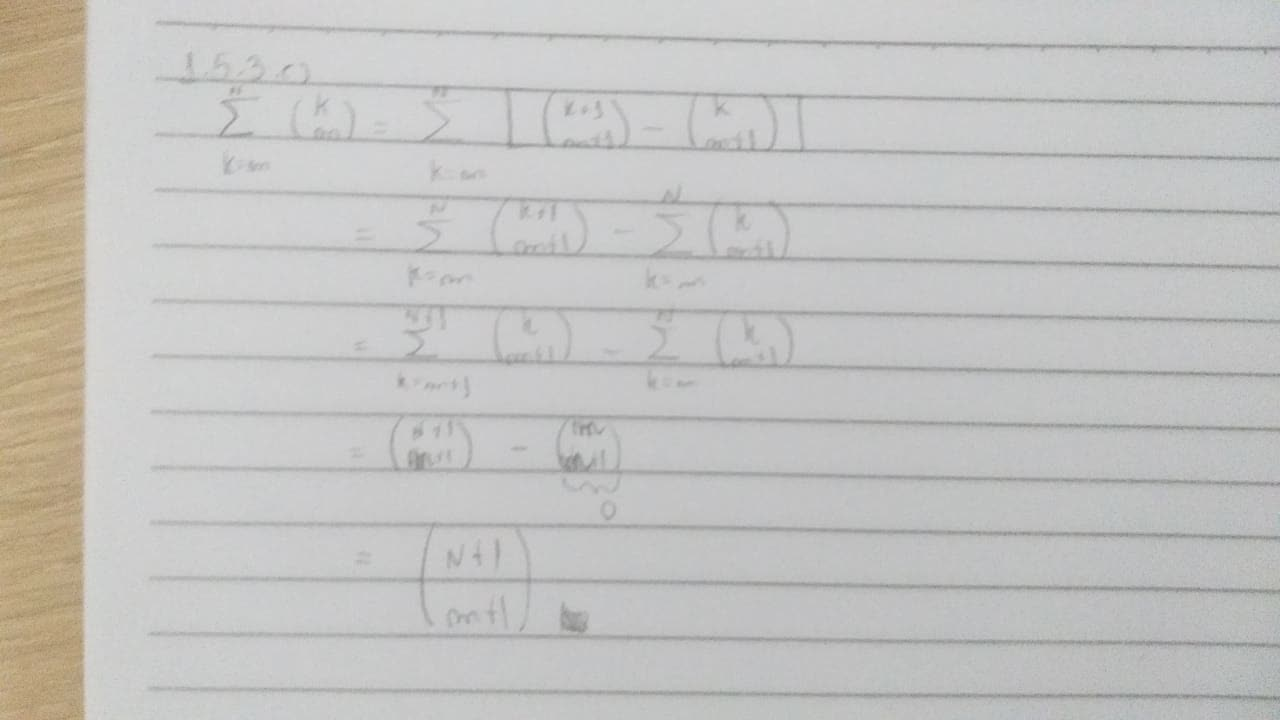
\includegraphics[width=0.8\textwidth]{images/153c.jpg}
				                  \caption{Questão 1.5.3 - c)}
			                  \end{figure}
		            \end{enumerate}
		      \item (1.5.6) Seja \(G\) um grafo qualquer com \(n\) vértices. Suponha, por contradição, que não existam dois vértices em \(G\) com o mesmo grau. Logo, como existem \(n\) vértices no grafo, os \(n\) possíveis graus que um vértice pode ter são \(\{0, 1, \dots, n-1\}\), logo podemos dizer que estes são os graus dos vértices de \(G\). No entanto, isso é absurdo, pois existiram um vértice de grau 0 e um vértice de grau \(n-1\) em um grafo com \(n\) vértices, o que não faz sentido. Logo, a premisa inicial estava errada, e podemos afirmar que todo grafo com \(n\) vértices, \(n \geq 2\), possui dois vértices com o mesmo grau.
		      \item (1.5.11) indução?
	      \end{itemize}
	\item \begin{itemize}
		      \item (2.8.3) Seja \(G\) um grafo com número cromático igual a \(\mathcal{X}(G)\). Sabemos que, para qualquer par de cores \(c_1, c_2\) da coloração mínima, deve existir ao menos uma aresta entre vértices \(v_1\), com cor \(c_1\), e \(v_2\), com cor \(c_2\). Caso contrário, todos os vértices com cor \(c_2\), poderiam ser coloridas com a cor \(c_1\) (sem perda de generalidade), o que seria contraditório com o fato da coloração ser mínima. Logo, para cada par de cores na coloração, deve existir ao menos uma aresta, e como cada aresta conecta exatamente dois vértices, temos que \(e(G) \ge \binom{\mathcal{X}(G)}{2}\).
		      \item (2.8.9) Seja \(G\) um grafo bipartido.
		      \item (2.8.15) A prova por ser feita por indução no número de arestas da árvore. A solução é trivial para o caso base em que \(e(T) = 1\). Para \(e(T) = 1\), \(T\) é uma aresta e trivialmente é subgrafo de qualquer grafo \(G\) com \(\delta(G) \geq 1\). Suponha que o resultado vale para qualquer árvore com \(k\) arestas. Seja \(T\) uma árvore qualquer com \(k + 1\) arestas e \(T' = T - \{v\}\) para alguma folha \(v \in V(T)\).
	      \end{itemize}

	\item

	      \begin{itemize}
		      \item (3.5.1)
		      \item (3.5.5)
		            %  e(g) > n^2/4  then g has at least floor(n/2) triangles
		            % 			for n = 1, 2, 3 trivial
		            %    				suppose true for k
		            % 			lets show for k+1
		            %    				suppose k+1 is even
		            %    				let v be an arbitrary vertex of g, remove it
		            % G - v has at least (k-1)/2 triangs. Adding v

		      \item (3.5.6)
		      \item (3.5.7)
		      \item (3.5.8)
		      \item (3.5.9)
	      \end{itemize}
\end{enumerate}

\end{document}
